\documentclass[a4paper,12pt]{book}

\usepackage{url}
\usepackage[utf8x]{inputenc}
\usepackage{amsmath}
\usepackage{graphicx}
\graphicspath{{images/}}
\usepackage{hyperref}
\usepackage{enumitem}
\usepackage{fancyhdr}

\usepackage[svgnames]{xcolor} % Required for colour specification
\newcommand*{\plogo}{\fbox{$\mathcal{MB}$}} % Generic dummy publisher logo

\usepackage{tikz,lipsum,lmodern}
\usepackage[most]{tcolorbox}

\def\checkmark{\tikz\fill[scale=0.4](0,.35) -- (.25,0) -- (1,.7) -- (.25,.15) -- cycle;}

\usepackage[extrafootnotefeatures]{xepersian}
\settextfont[Scale=1.1]{B Nazanin}
\setlatintextfont[Scale=1]{Times New Roman}

%\linespread{1.3} %line spacing

% Header
\pagestyle{fancy}
% with this we ensure that the chapter and section
% headings are in lowercase.
\renewcommand{\chaptermark}[1]{%
	\markboth{#1}{}}
\renewcommand{\sectionmark}[1]{%
	\markright{\thesection\ #1}}
\fancyhf{} % delete current header and footer
\fancyhead[LE,RO]{\bfseries\thepage}
\fancyhead[LO]{\bfseries\rightmark}
\fancyhead[RE]{\bfseries\leftmark}
\renewcommand{\headrulewidth}{0.5pt}
\renewcommand{\footrulewidth}{0pt}
\addtolength{\headheight}{0.5pt} % space for the rule
\fancypagestyle{plain}{%
	\fancyhead{} % get rid of headers on plain pages
	\renewcommand{\headrulewidth}{0pt} % and the line
}

\begin{document}

%----------------------------------------------------------------------------------------
%	TITLE PAGE
%----------------------------------------------------------------------------------------

\begin{titlepage} % Suppresses headers and footers on the title page
	
	\centering % Centre all text
	
	%------------------------------------------------
	%	Title and subtitle
	%------------------------------------------------
	
	\setlength{\unitlength}{0.6\textwidth} % Set the width of the curly brackets above and below the titles
	
	{\color{LightGoldenrod}\resizebox*{\unitlength}{\baselineskip}{\rotatebox{90}{$\}$}}}\\[\baselineskip] % Top curly bracket
	
	\textcolor{Sienna}{\textit{\Huge \lr{Spring Cloud}}}\\[\baselineskip] % Title
	
	%{\color{RosyBrown}\Large }\\ % Subtitle or further description
	
	{\color{LightGoldenrod}\resizebox*{\unitlength}{\baselineskip}{\rotatebox{-90}{$\}$}}} % Bottom curly bracket
	
	\vfill % Whitespace between the title and the author name
	
	%------------------------------------------------
	%	Author
	%------------------------------------------------
	
	{\Large\lr{Milad Barzideh}}\\ % Author name
	
	\vfill % Whitespace between the author name and the publisher logo
	
	%------------------------------------------------
	%	Publisher
	%------------------------------------------------
	
	\plogo\\[0.5\baselineskip] % Publisher logo
	
     % Publisher name
	
\end{titlepage}

\tableofcontents

%----------------------------------------------------------------------------------------
%	Content
%----------------------------------------------------------------------------------------

\chapter{میکروسرویس‌ها، ابر و چیزهای دیگر}

میکروسرویس‌‌  یا ریزخدمت\LTRfootnote{Microservice}
یکی از اصطلاحاتی‌ست که این روزها در دنیای نرم‌افزار رایج شده است. میکروسرویس‌‌ها، سرویس‌هایی توزیع‌شده و مجزا هستند که هر کدام از آن‌ها وظیفه‌ی کوچک و مشخصی را انجام می‌دهند. در این نوشتار، پس از معرفی میکرسرویس‌ها و ذکر  مشخصه‌های آن،‌ با استفاده از فریمورک‌های 
\lr{Spring Boot} 
و
\lr{Spring Cloud}
به صورت عملی، معماری میکروسرویس‌ها را بررسی خواهیم کرد.

\section{میکروسرویس چیست؟}
قبل از مطرح شدن میکروسرویس‌ها بیشتر برنامه‌های تحت‌وب با استفاده از معماری یکپارچه\LTRfootnote{Monolithic}
ساخته می‌شدند. در معماری یکپارچه، هر برنامه به عنوان یک محصول نرم‌افزاری قابل اجرا در نظر گرفته می‌شود و رابط کابری، منطق برنامه و دسترسی به پایگاه داده، همه در یک برنامه‌ی کاربردی قرار گرفته می‌شود. 

هر برنامه به عنوان یک واحد کاری در نظر گرفته می‌شود که معمولا چندین تیم توسعه روی بخش‌های مختلف آن کار می‌کنند. یکی از مشکلاتی که در این حالت پیش می‌آید این است که با افزایش اندازه و پیچیدگی برنامه،‌ هزینه‌های ارتباطی و هماهنگی تیم‌ها، بیشتر و سخت‌تر می‌شود. برای مثال با هر تغییری که تیم‌ها ایجاد می‌کنند، کل برنامه دوباره باید تست و مستقر\LTRfootnote{Redeployed} شود. 

مفهوم میکروسرویس تقریبا از سال 2014 و در پاسخ به چالش‌هایی که برای مقیاس‌پذیر کردن برنامه‌های یکپارچه وجود داشت، وارد جامعه‌ی نرم‌افزار شد. همان‌طور که گفته شد یک میکروسرویس، کوچک، مجزا و توزیع‌شده است. بنابراین این امکان را فراهم می‌کند که برنامه‌های بزرگ را به بخش‌های کوچکتری تقسیم کرد تا مدیریت و توسعه‌ی آن‌ها آسان‌تر داده شوند. مهم‌ترین نکته‌ای که باید به آن توجه داشته باشید، تجزیه و جداسازی عملکردهای برنامه است به صورتی که کاملا مستقل از همدیگر باشند. 

\begin{figure}[h]
	\centering
	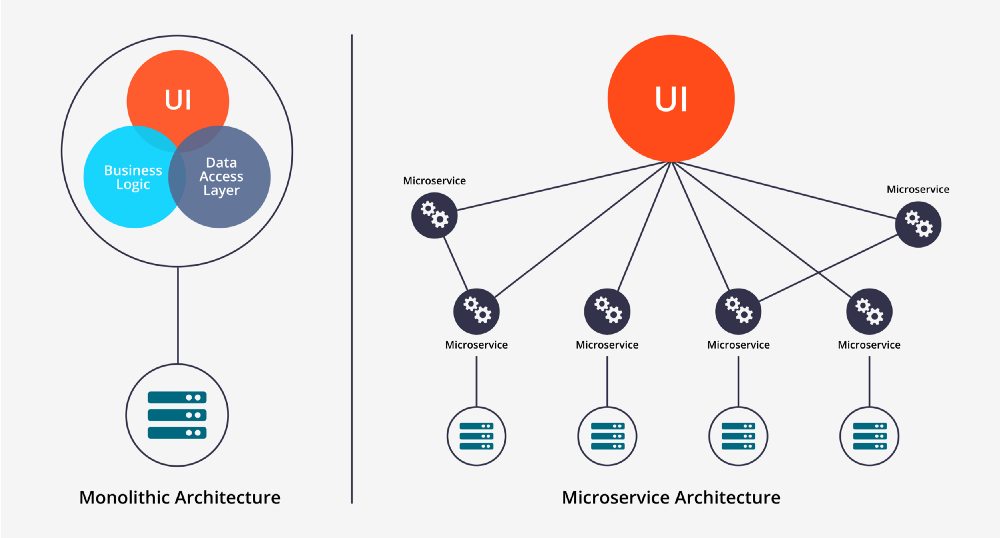
\includegraphics[width=\textwidth]{1.png}
	\caption{ معماری یکپارچه در مقابل معماری میکروسرویس}
	\label{fig:1}
\end{figure}

همان‌طور که شکل \ref{fig:1} نشان می‌دهد هر تیم می‌تواند کدها و زیرساخت مربوط به سرویس خود را داشته باشد و آن‌ها را به صورت مستقل نسبت‌ به سرویس‌های دیگر توسعه و ارزیابی کند.

\vskip 0.3cm
معماری میکروسرویس ویژگی‌های زیر را دارد:
\begin{itemize}[label=$\ast$]
		\item  منطق برنامه به قسمت‌های کوچک‌تر شکسته می‌شود که هر قسمت مسئله‌ی مشخص و تعریف شده‌ای را حل می‌کند.
	\item هر قسمت محدوده‌ی مسئولیت مشخصی دارد و مستقل از سایر بخش‌ها توسعه و استقرار می‌یابد. همچنین میکروسرویس‌ها باید قابلیت استفاده‌ی مجدد در برنامه‌های دیگر را داشته باشند.
	\item میکروسرویس‌ها با استفاده از قواعد مشخص و بکارگیری پروتکل‌های ارتباطی سبک‌وزن مانند \lr{HTTP} و 
	\lr{JSON}
	داده‌ها را مبادله می‌کنند.
	\item پیاده‌سازی فنی هر میکروسرویس بی‌اهمیت است؛ زیرا برنامه‌ها با پروتکل‌های مستقل از تکنولوژی\LTRfootnote{Technology-neutral protocol}
	با هم ارتباط برقرار می‌کنند. این یعنی برنامه‌‌ای که با معماری میکروسرویس ساخته شده می‌تواند از تکنولوژی‌ها و زبان‌های مختلفی استفاده کند. 
	\item میکروسرویس‌ها برای سازمان‌ها این امکان را فراهم می‌کنند که تیم‌های توسعه‌ی کوچک با وظایف کاری مشخص داشته باشند.
\end{itemize} 


\section{محاسبات ابری چیست؟}



\section{چرا ابر؟}

به عنوان یک توسعه‌دهنده‌ی میکروسرویس، دیر یا زود باید تصمیم بگیرید سرویس‌تان را در یکی از جاهای زیر مستقر کنید:
\begin{itemize}[label=$\ast$]
	\item \textit{سرور فیزیکی:} 
	سازمان‌های کمی این کار را انجام می‌دهند؛ زیرا سرورهای فیزیکی محدودیت ایجاد می‌کنند. برای مثال شما نمی‌توانید ظرفیت سرور فیزیکی را سریعا افزایش دهید یا میکروسرویس را به دلیل هزینه‌هایی زیادی که در پی دارد روی چندین سرور فیزیکی مستقر کنید.
	

	\item \textit{ماشین مجازی:}
	یکی از مهم‌ترین فواید میکروسرویس‌ها، توانایی آن‌ها در افزودن یا کاهش نمونه‌های یک سرویس است (مقیاس‌پذیری). یک میکروسرویس  را می‌توان در یک ماشین مجازی قرار داد و به آسانی چندین نمونه از آن را روی زیرساخت‌های موجود مستقر کرد.
	
	\item \textit{ظرف مجازی\LTRfootnote{Virtual container}:} 
	به جای استقرار میکروسرویس ‌روی یک ماشین مجازی کامل، بسیاری از توسعه‌دهندگان سرویس‌های خود را به صورت ظرف‌های داکر\LTRfootnote{Docker}
در محیط ابری مستقر می‌کنند. 
\end{itemize}


\href{https://nickjanetakis.com/blog/comparing-virtual-machines-vs-docker-containers}
{ تفاوت داکر با ماشین مجازی}

\vskip 0.5cm
مزیت مهم میکروسرویس‌های تحت ابر انعطاف‌پذیری بالای آن‌هاست. ارائه‌دهندگان محیط ابری اجازه می‌دهند در کم‌تر از چند دقیقه یک ماشین مجازی یا یک ظرف جدید را اضافه یا حذف کنید. همچنین برنامه‌ها مقاوم‌تر هستند، برای مثال اگر یکی از میکروسرویس‌ها از کار بیفتد می‌توان از نمونه‌های دیگر آن میکروسرویس استفاده کرد و برنامه را بالا نگه داشت. 











\chapter{کنترل پیکربندی‌ها}
به عنوان یک توسعه‌دهنده می‌دانید که
\lr{hard-code} 
کردن مقادیر در کدهای برنامه چندان منطقی نیست، به همین دلیل معمولا توسعه‌دهندگان از یک فایل ثابت استفاده می‌کنند و همه اطلاعات پیکربندی برنامه را در آن قرار می‌دهند. با این حال قرار دادن این اطلاعات در کدهای برنامه مشکل‌ساز است، زیرا با هر تغییر در پیکربندی، کل برنامه دوباره باید کامپایل شود. برای جلوگیری از این کار، توسعه‌دهندگان اطلاعات مربوط به پیکربندی را از کدهای برنامه جدا می‌کنند. 

این مشکل در برنامه‌های تحت ابر بیشتر خود را نشان می‌دهد، از آن‌جا که ممکن است این برنامه‌ها از صدها میکروسرویس با چندین نمونه‌ی در حال اجرا تشکیل شده باشند، مدیریت پیکربندی برنامه بسیار مشکل است. برای همین توسعه‌ی میکروسرویس‌های تحت ابر روی موارد زیر تاکید دارد:
\begin{enumerate}
	\item جداسازی پیکربندی برنامه از کدهای اصلی برنامه که باید مستقر شوند.
	\item تزریق اطلاعات مربوط به پیکربندی برنامه در زمان راه‌اندازی سرور با استفاده از یک مخرن مرکزی به میکروسرویس‌‌های برنامه.
\end{enumerate}


\section{معماری مدیریت پیکربندی}


\section{روش‌های پیاده‌سازی}


\begin{tcolorbox}[colback=red!5!white,colframe=red!75!black]
	
\end{tcolorbox}



















\end{document}
